\section{Разработка спецификации требований}
\label{sec:domain}

\subsection{Разработка спецификации функциональных требований}
\label{sec:domain:specification}

По результатам анализа предметной области и существующих аналогов можно сделать вывод, что проектируемое программное средство должно поддерживать ряд функций для снижения временных затрат пользователя на ведение своей бухгалтерии, ключевыми из которых являются следующие:

\begin{itemize}
	\item работа с категориями (создание, изменение, удаление, выбор типа, валюты, названия);
	\item добавление операции в категории;
	\item уведомление пользователя о приближении к заданному порогу трат;
	\item вывод статистики по категориям;
	\item очистка статистики за последний месяц в каждом новом месяце.
\end{itemize}

С учетом требований, определенных в подразделе \ref{sec:analysis:specification}, определяется детализацию функций проектируемого ПС.

\subsubsection{} Старт диалога с ботом
\label{sec:domain:specification:startdialog}

Требования к реализации функции:

\begin{enumerate}
	\item После команды start в диалоге бота, должна произойти проверка на существование пользователя в базе данных.
	\item В случае отсутствия пользователя в базе, пользователь должен быть создан и добавлен в базу с двумя стандартными категориями, одной для доходов, второй для расходов, а также с обнуленным контекстом пользователя.
	\item Далее должен быть показан список функций бота.
\end{enumerate}

\subsubsection{} Добавление категории
\label{sec:domain:specification:addcategory}

Требования к реализации функции:

\begin{enumerate}
	\item После инициализации процесса бот должен инициализировать контекст пользователя и начать диалог с пользователем для настройки категории.
	\item Для успешной настройки категории пользователь должен указать тип категории, валюту, название категории, а также желаемый порог расходов для исходящих категорий.
	\item Необходима обработка неправильных, либо не подходящих по контексту команд. Если такая команда попадает на обработку, пользователю должно быть отправлено сообщение о том, что команда не может быть обработана.
	\item При команде отмена от пользователя, контекст пользователя должен быть очищен, а вновь созданная категория должна быть удалена из базы. После очистки, пользователю должен быть показан список функций бота.
	\item При успешном добавлении категории, контекст пользователя должен быть очищен, вновь созданная категория должна быть переведена в состояние configured. Пользователю должен быть показан список функций бота.
\end{enumerate}

\subsubsection{} Изменение категории
\label{sec:domain:specification:editcategory}

Требования к реализации функции:

\begin{enumerate}
	\item После инициализации процесса бот должен инициализировать контекст пользователя и начать диалог с пользователем для настройки категории.
	\item Пользователь должен выбрать, какую категорию он хотел бы изменить.
	\item После выбора категории, пользователь должен перейти к настройке категории, аналогично функции создания.
	\item Для успешной настройки категории, пользователь должен указать тип категории, валюту, название категории, а также желаемый порог расходов для исходящих категорий.
	\item При команде отмена от пользователя, категория должна быть сохранена в состоянии, в котором ее успел изменить пользователь. Контекст пользователя должен быть очищен, а также должен быть показан список функций бота.
	\item При успешном изменении категории, контекст пользователя должен быть очищен, категория должна быть сохранена. Пользователю должен быть показан список функций бота.
\end{enumerate}

\subsubsection{} Удаление категории
\label{sec:domain:specification:deletecategory}

Требования к реализации функции:

\begin{enumerate}
	\item После инициализации процесса бот должен инициализировать контекст пользователя и начать диалог с пользователем для удаления категории.
	\item Пользователь должен выбрать, какую категорию он хотел бы удалить.
	\item После выбора категории, она должна быть удалена, контекст пользователя должен быть очищен, пользователю должен быть показан список функций бота.
	\item При команде отмена от пользователя, контекст пользователя должен быть очищен, а также должен быть показан список функций бота.
\end{enumerate}

\subsubsection{} Добавление операции в категорию
\label{sec:domain:specification:addoperationtocategory}

Требования к реализации функции:

\begin{enumerate}
	\item После инициализации процесса бот должен инициализировать контекст пользователя и начать диалог с пользователем для добавления операции.
	\item Пользователь должен выбрать, в какую категорию он хочет добавить операцию.
	\item После выбора категории, пользователь должен перейти к настройке операции.
	\item Для успешной настройки операции, пользователь должен указать сумму операции, а также дату операции.
	\begin{enumerate}
		\item Пользователь может ввести дату вручную в определенном формате.
		\item При желании, пользователь может воспользоваться кнопкой <<now>>. В таком случае, операции будет присвоена текущие дата и время.
	\end{enumerate}
	\item При команде отмена от пользователя, контекст пользователя должен быть очищен, а вновь созданная операция должна быть удалена из базы. После очистки, пользователю должен быть показан список функций бота.
	\item При добавлении операции в категорию-расход, если пользователь превысил или близок к тому, чтобы превысить порог, настроенный для категории, должно быть отправлено соответствующее сообщение.
	\item При успешном добавлении операции в категорию, контекст пользователя должен быть очищен, вновь созданная операция должна быть переведена в состояние configured. Пользователю должен быть показан список функций бота.
\end{enumerate}

\subsubsection{} Просмотр статистики для всех категорий
\label{sec:domain:specification:showallstats}

Требования к реализации функции:

\begin{enumerate}
	\item После инициализации процесса бот должен показать пользователю список категорий с суммами их операций.
	\begin{enumerate}
		\item Если категория является категорией-доходом, сумма должна быть отображена со знаком плюс.
		\item Если категория является категорией-расходом, сумма должна быть отображена со знаком минус.
	\end{enumerate}
\end{enumerate}

\subsubsection{} Просмотр статистики для входящих категорий
\label{sec:domain:specification:showincomestats}

Требования к реализации функции:

\begin{enumerate}
	\item После инициализации процесса бот должен показать пользователю список категорий с суммами их операций.
	\item Сумма должна быть отображена со знаком плюс.
\end{enumerate}

\subsubsection{} Просмотр статистики для исходящих категорий
\label{sec:domain:specification:showexpensestats}

Требования к реализации функции:

\begin{enumerate}
	\item После инициализации процесса бот должен показать пользователю список категорий с суммами их операций.
	\item Сумма должна быть отображена со знаком минус.
\end{enumerate}

\subsubsection{} Просмотр статистики для конкретной категории
\label{sec:domain:specification:showcustomcategorystats}

Требования к реализации функции:

\begin{enumerate}
	\item После инициализации процесса бот должен инициализировать диалог для выбора пользователем категории.
	\item При команде отмена от пользователя, контекст пользователя должен быть очищен. После очистки, пользователю должен быть показан список функций бота.
	\item После выбора категории, пользователь должен получить список операций с указанием суммы и даты добавления операции.
	\begin{enumerate}
		\item Если категория является категорией-доходом, сумма должна быть отображена со знаком плюс.
		\item Если категория является категорией-расходом, сумма должна быть отображена со знаком минус.
	\end{enumerate}
\end{enumerate}

\subsection{Варианты использования программного средства} 
\label{sec:domain:model:use_cases}

Use case диаграмма, разработанная с использованием нотации \linebreak \uml, представлена на рисунке \ref{fig:domain:model:use_cases:model}.

\begin{figure}[!h]
\centering
	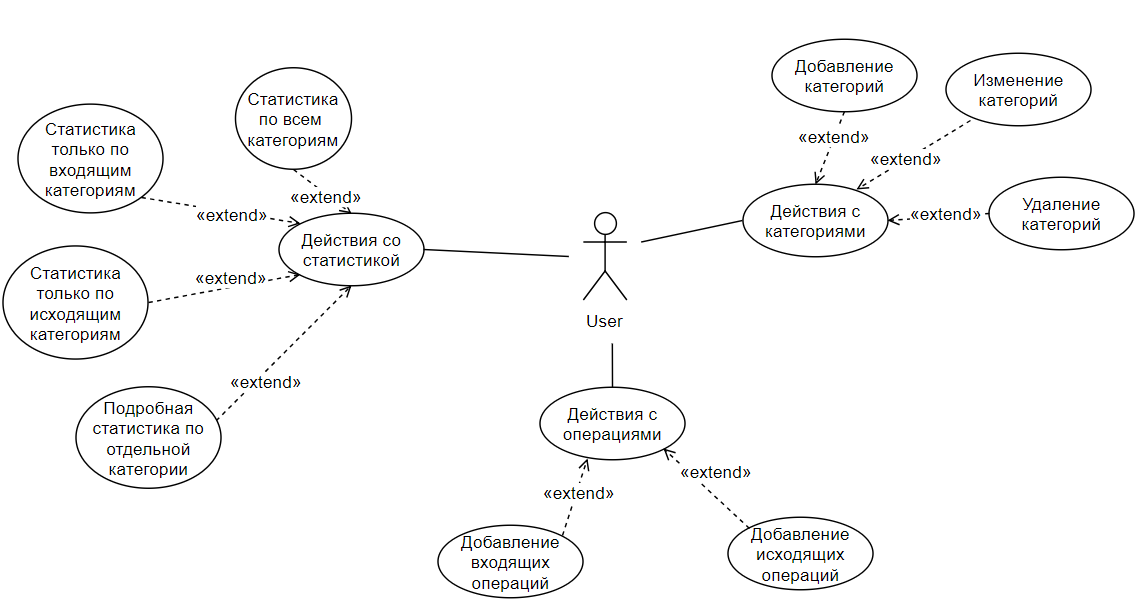
\includegraphics[scale=0.4]{use_case.png}
	\caption{Use case диаграмма ПС}
	\label{fig:domain:model:use_cases:model}
\end{figure}

Подробное описание указанных на рисунке прецедентов представлено ниже.

Добавление категорий -- функция, с помощью которой пользователь может добавить категорию, а также настроить ее по своему усмотрению. После вызова функции добавления категории, должен начаться диалог, в котором приложение последовательно будет задавать вопросы по каждому из пунктов настройки категории. Во время диалога пользователь может вызвать команду отмены. Для завершения диалога настройки, пользователь должен указать тип категории, имя категории, а также валюту. Для категорий расходов пользователь также должен указать желаемый порог расходов.

Изменение категорий происходит по такому же сценарию, как и в случае создания. При вызове функции пользователь должен выбрать категорию для изменения. Далее начинается диалог изменения.

Для удаления категорий пользователь должен выбрать категорию для удаления.

Добавление входящих операций -- функция, с помощью которой пользователь может добавить операцию в одну из категорий-доходов. После вызова функции пользователь должен выбрать категорию для добавления операции. Далее приложение инициализирует диалог добавления операции. Пользователь может отменить создание операции с помощью команды отмены. Для добавления операции в категорию-доход пользователю требуется ввести сумму в валюте категории, а также указать дату. Пользователь может ввести дату вручную, либо нажать кнопку <<now>>.

Добавление исходящих операций -- функция, с помощью которой пользователь может добавить операцию в одну из категорий-расходов. Функция отличается от функции добавления входящих операций тем, что после ввода суммы в валюте категории, приложение уведомляет пользователя о скором достижении установленного порога расходов.

Функция просмотра статистики по всем категориям позволяет пользователю просматривать статистику доходов и расходов по всему списку категорий. В этом случае на выход пользователю будет предоставлен список из названия категории, а также сумма операций со знаком плюс для категорий-доходов и со знаком минус для категорий-расходов.

Функция просмотра статистики по входящим категориям идентична предыдущей, за исключением того, что она предоставляет только список категорий доходов, без категорий-расходов.

Функция просмотра статистики по исходящим категориям идентична предыдущей, за исключением того, что она предоставляет только список категорий расходов, без категорий-доходов.

Подробная статистика со всеми операциями предоставляется пользователю функцией просмотра подробной статистики отдельной категории. При вызове функции пользователь получает список операций в этой категории, вместе с суммой по операции, а также датой добавления.

\subsection{Разработка инфологической модели базы данных}
\label{sec:domain:model:db}

Исходя из необходимости использования в проектируемом приложении базы данных, разработаем ее инфологическую модель. Для ее создания будем использовать расширение диаграммы классов \uml, предназначенное для моделирования баз данных. Полученная диаграмма (рисунок \ref{fig:domain:model:db:model}) будет являться моделью базы данных инфологического уровня \cite{kulikov_db_workbook}.

\begin{sidewaysfigure}
\centering
	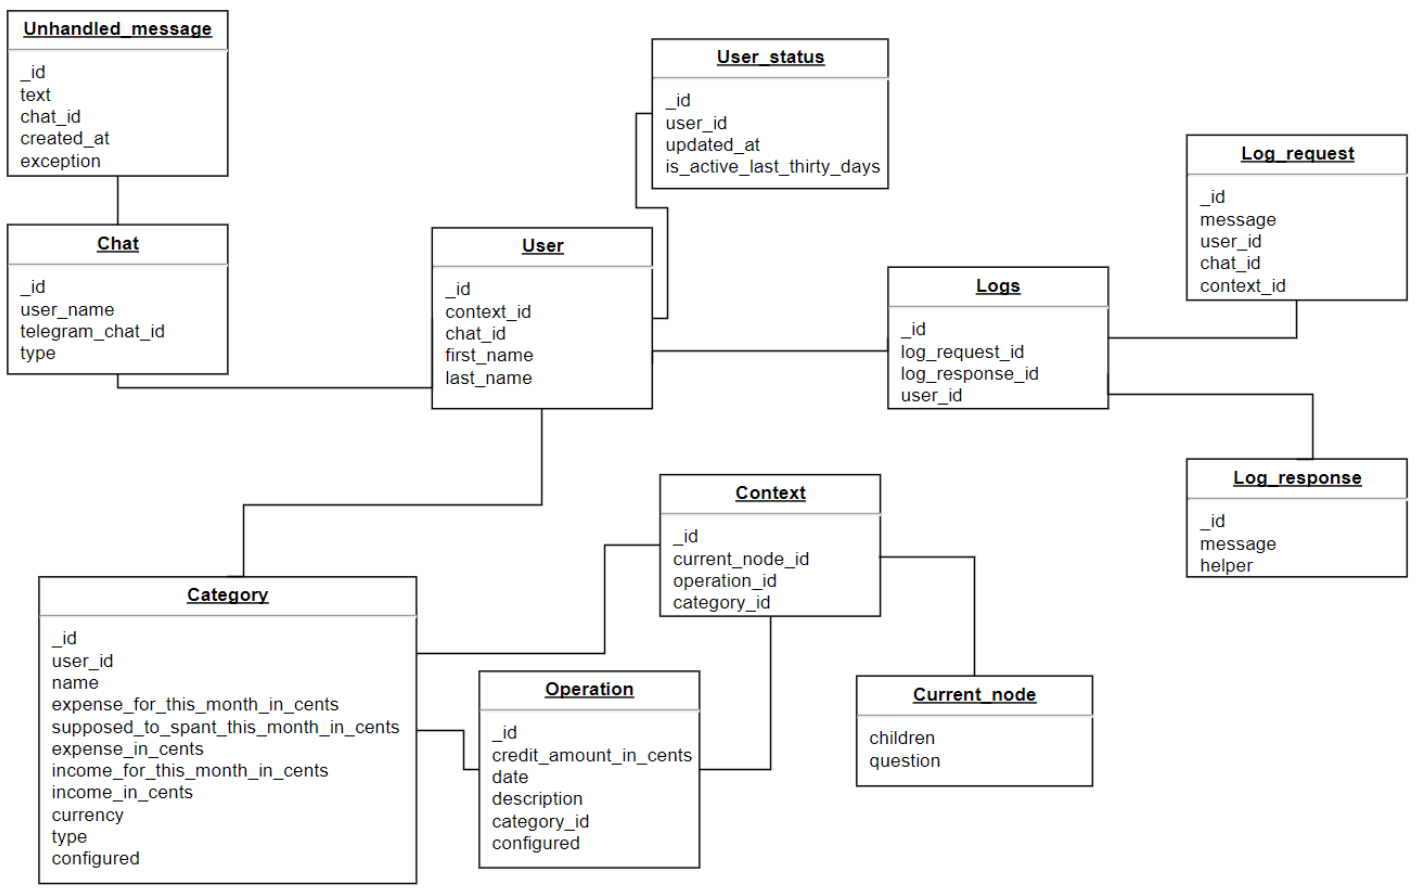
\includegraphics[scale=0.65]{db_schema.png}
	\caption{Инфологическая модель базы данных}
	\label{fig:domain:model:db:model}
\end{sidewaysfigure}

Схема базы данных построена на существующей модели, использующейся на платформе Telegram Bots.

В силу того, что для платформы Telegram Bots не нужно дополнительно авторизовываться, в таблице User отсутствует поле для хешированного пароля. Также, сущность пользователя хранит в себе так называемый контекст пользователя. Контекст требуется для сохранения состояния диалога между пользователем и ботом во время настройки категорий и добавления операций, а также просмотра статистики.

Сущность Unhandled message используется для хранения сообщений об ошибках пользователей, связанных с неправильно обработанными командами, полученными ботом.

Сущность Chat хранит в себе информацию о чате между ботом и пользователем, а также его состояние.

\newpage

Сущность Category хранит в себе информацию о категории, включая суммы по доходам/расходам за текущий месяц, а также за все время. Поле configured отвечает за состояние конфигурации категории. Если категория не сконфигурирована и пользователь отправляет боту команду отмены, категория удаляется из базы данных.

Сущность Operation хранит в себе информацию о конкретной операции, включая сумму, дату добавления и описание. Поле configured отвечает за состояние конфигурации операции. Если операция не сконфигурирована и пользователь отправляет боту команду отмены, операция удаляется из базы данных.

Сущность Context хранит в себе информацию о текущем контексте диалога между пользователем и ботом. Представляет собой древовидную структуру, с помощью которой бот узнает о том, на какой вопрос пришел ответ от пользователя.

Помимо всего прочего, в схеме базы данных имеются сущности, использующиеся для логирования запросов пользователя и ответов бота. За это отвечают сущности Log request и Log response.